\chapter*{Design Problem}

\section*{Nomenclature}
\begin{tabular}[t]{p{0.05\textwidth}p{0.4\textwidth}}
	$ C_a $ & number of shift daily, $ \unit{shifts} $\\
	$ K_{ng} $ & working days/year, $ \unit{days} $\\
	$ L $ & service life, $ \unit{years} $\\
	$ n $ & rotational velocity of the mixing tank, $ \unit{rpm} $\\	
\end{tabular}
\begin{tabular}[t]{p{0.05\linewidth}p{0.4\linewidth}}
	$ P $ & design power of the mixing tank, $ \unit{kW} $\\
	$ T_1 $ & working torque 1, $ \unit{N\cdot m} $\\
	$ T_2 $ & working torque 2, $ \unit{N\cdot m} $\\
	$ t_1 $ & working time 1, $ \unit{s} $\\
	$ t_2 $ & working time 2, $ \unit{s} $\\
\end{tabular}

\section{Problem}
The problem is downloaded from E-learning website, designated number 8, see Figure \ref{fig:problem}.
\begin{figure}[ht]
	\centering
	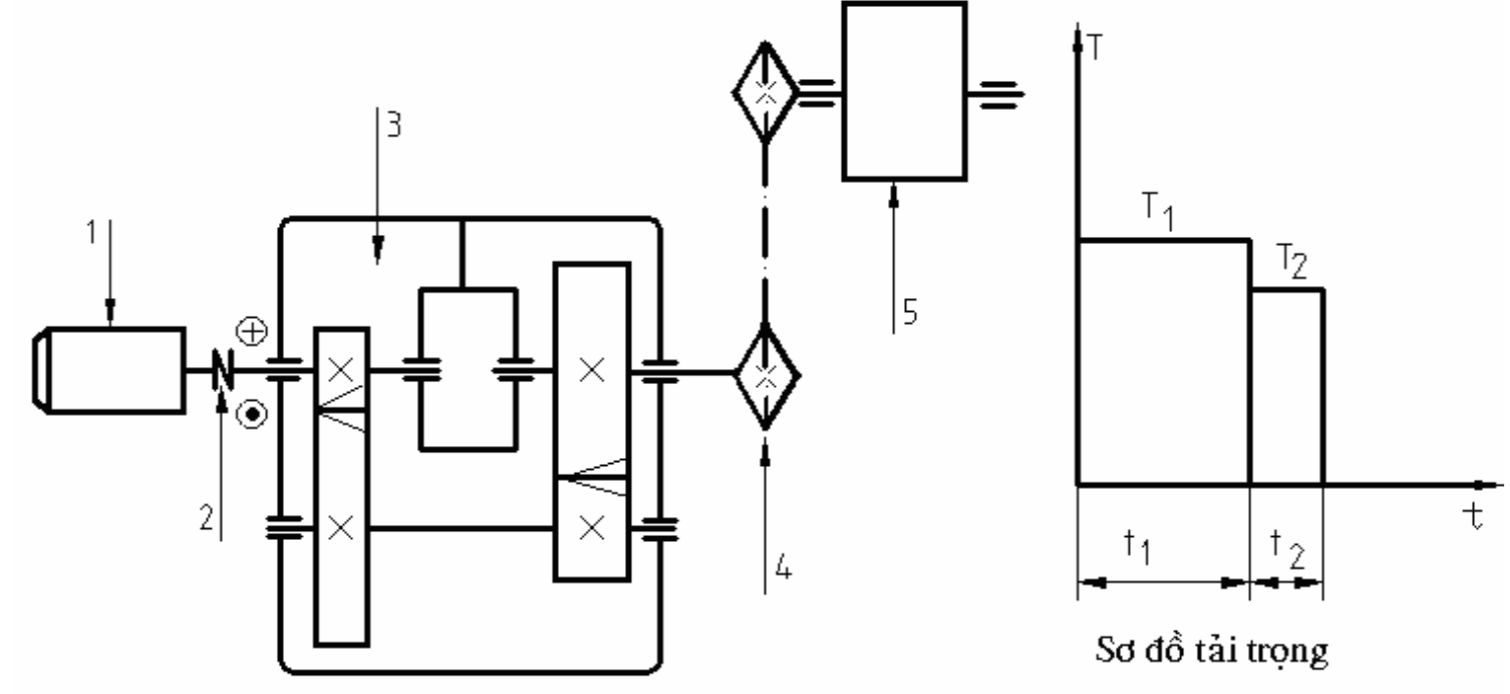
\includegraphics[width=\linewidth]{images/problem}
	\caption{Working principle diagram and workload of the mixing machine: 1) electric motor, 2) elastic coupling, 3) two-stage coaxial helical speed reducer, 4) roller chain drive, 5) mixing tank (one-directional, light duty, operate 1 shift, 8 hours each)}
	\label{fig:problem}
\end{figure}

\section{Mixing machine parameters}
From the parameters given in the document, we have:\\
\begin{tabular}{p{0.4\linewidth}p{0.4\linewidth}}
	$ P=7 \unitp{kW}$ & $ t_1=15\unitp{s} $\\
	$ n=65\unitp{rpm} $ & $ t_2=11\unitp{s} $\\
	$ L=8\unitp{years} $ & $ T_1=T\unitp{N\cdot m} $\\
	$ K_{ng}=260\unitp{days} $ & $ T_2=0.7T\unitp{N\cdot m} $\\
	$ Ca=1\unitp{shifts} $&\\
\end{tabular}

\section{Requirements}
\begin{itemize}
	\item 01 report.
	\item 01 assembly drawing.
	\item 01 detailed drawing.
\end{itemize}

\section{Design problem}
\begin{enumerate}
	\item Decide the working power of the electric motor and transmission ratio of the system.
	\item Calculate and design machine elements:
	\begin{enumerate}
		\item Calculate system drives (belt, chain or gear).
		\item Calculate the elements in speed reducers (gears, lead screws).
		\item Draw and calculate force diagram exerting on the transmission elements.
		\item Calculate, design shafts and keys.
		\item Choose bearings and couplings.
		\item Choose machine bodies, fasteners and other elements.
	\end{enumerate}
	\item Choose assembly tolerance.
	\item Bibliography
\end{enumerate}
